% !TEX root = ../main.tex
%

\section{Results}



\subsection{Our proposed strategy significantly improves synthetic discussions}

Figure \ref{fig::strategy_barplot} shows the aggregated scores for each moderation strategy, while Figure \ref{fig::toxicity_aq_stats} displays the mean difference between annotated toxicity and argument quality respectively, given each moderation strategy. Discussions where a moderator is absent feature overall significantly increased toxicity and decreased argument quality. In general, while most strategies lead to statistically significant effects on both measures (Kruskal-Wallis $p=0$ for both measures), the qualitative difference is relatively small, especially when it comes to argument quality.

However, some strategies seem to have a qualitatively significant impact on discussions. Our proposed “Moderation Game” strategy (see Section \ref{ssec:setup:strategies}) outperforms all baselines (“No Moderator”, “Moderator without strategy”, “Rules-only”), as well as the other established strategies (“Moderation guidelines”, “Facilitation guidelines”) by a smaller margin. This is more evident when looking at toxicity.
In fact, contrary to our expectations, these widely used guidelines do not seem to outperform even the “Rules Only” strategy (which does not include any instructions on how the \ac{LLM} moderator can achieve effective moderation).

\begin{figure*}[t]
	\centering
	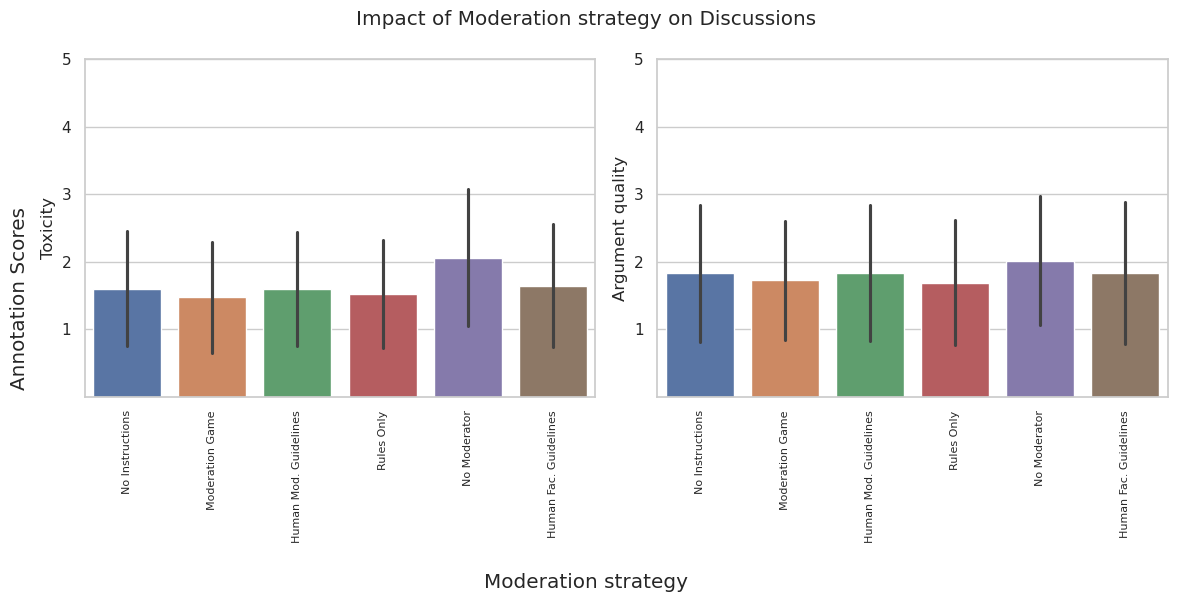
\includegraphics[width=\linewidth]{strategy_barplot.png}
	\caption{Effects of moderation strategy for toxicity and argument quality. Error bars represent the 95\% confidence interval. Less is better (e.g., Argument Quality = 1 represents very high quality discussions).}
	\label{fig::strategy_barplot}
\end{figure*}

\begin{figure*}[t]
    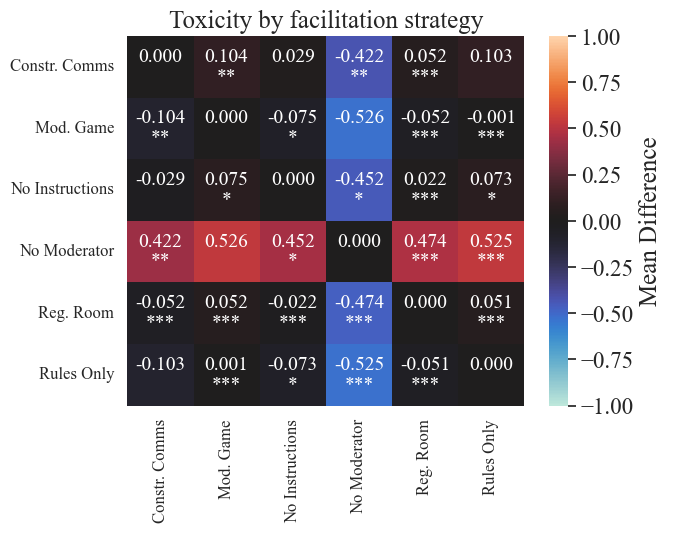
\includegraphics[width=0.48\linewidth]{toxicity_stats.png} \hfill
    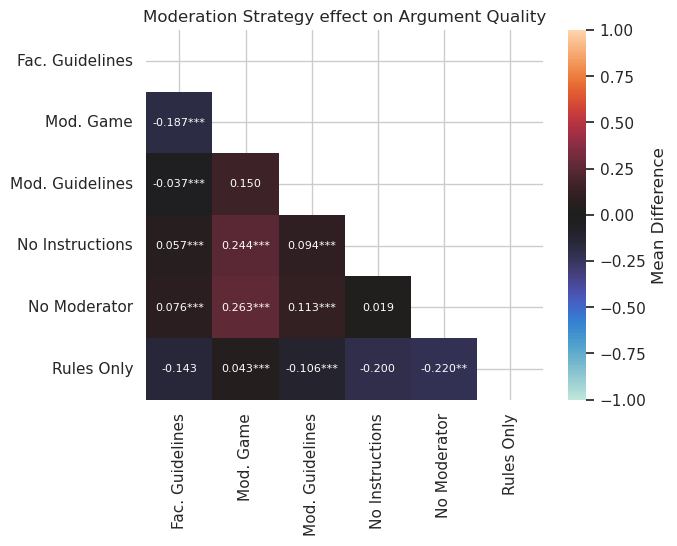
\includegraphics[width=0.48\linewidth]{argumentq_stats.png}
	\centering
	\caption{Mean difference of Toxicity (left) and Argument Quality (right) between each moderation strategy. $A[i, j] = 0.3^{***}$ indicates that the strategy $j$ is better than the strategy $i$ for an average of $0.3$ points with $p<0.001$. Each comparison is accompanied by Dunn's posthoc test for multiple comparisons \cite{dunn}, in the form of significance asterisks.}
	\label{fig::toxicity_aq_stats}
\end{figure*}


\subsection{LLM moderators intervene at almost any opportunity.}

As demonstrated by Figure \ref{fig::intervention_count}, \ac{LLM} moderators will respond at almost every point in the discussion. We also observe that \ac{LLM} user-agents are unusually lenient towards repeated, unneeded interventions of moderators, which is not representative of human behavior. In this situation, human users tend to get irritated, and we can usually observe a rise in toxicity \cite{schaffner_community_guidelines, make_reddit_great, proactive_moderation, cresci_pesonalized_interventions}.


\subsection{LLM user-agents instructed to behave like trolls contribute negatively to the discussions}

Unsurprisingly, comments from \ac{LLM} user-agents with the intent to act as trolls feature significantly higher toxicity and polarization scores, while also featuring the lowest quality arguments (Figure \ref{fig::intent_barplot}). We do not find a significant difference in toxicity between the neutral and community-driven user-intents (see Section \ref{ssec:experimental:discussions}), however.


\subsection{LLM annotators exhibit some disagreement, and disagree more on Argument Quality}

Figure \ref{fig::annotator_variance} displays the average variance for the comments of each discussion. As reported by \citet{argyle2023}, \ac{LLM} annotators disagree more on Argument Quality, which is likely due to its less clear definition, compared to Toxicity.


\subsection{The choice of LLM has a significant impact on the variety of the synthetic discussions}

We follow the example of \citet{ulmer2024bootstrappingllmbasedtaskorienteddialogue} and use average pairwise F1 ROUGE-L scores \cite{lin-2004-rouge} to gauge diversity in the synthetic discussions. Intuitively, this measure estimates the maximum number of common n-grams between all comments in each discussion. The use of n-grams instead of other text-based similarity measures (such as embedding cosine similarity) is important, since \ac{LLM} discussions tend to lack linguistic variety even on the level of individual words and sentences \cite{ulmer2024bootstrappingllmbasedtaskorienteddialogue}. 

Figure \ref{fig::discussion_variance} demonstrates that the Qwen-2.5 model features the largest amount of variance (low average ROUGE-L scores), while LLaMa-3.1 struggles the most to create varied responses. The latter can be also verified qualitatively; LLaMa-based user-agents tend to behave in a stereotypically polite and inoffensive fashion. Additionally, Figure \ref{fig::comment_length} shows that different \acp{LLM} gravitate towards different lengths in their comments. Qwen-2.5 produces relatively shorter comments (with relatively little variance), while LLaMa-3.1's are almost double the size on average.

These results indicate that a larger \ac{LLM} may not necessarily lead to more authentic or varied discussions. We posit that models subjected to intense alignment procedures, may not be able to replicate human behavior as authentically as other models. This finding has also been reported by \citet{Park2023GenerativeAI}. However, we note that the abliterated model, which was supposed to be more resistant to alignment artifacts, does not exhibit significantly more toxicity (Figure \ref{fig::model_barplot}), unlike what would have been expected (see Section \ref{ssec:experimental:technical}).

\begin{figure}
	\centering
	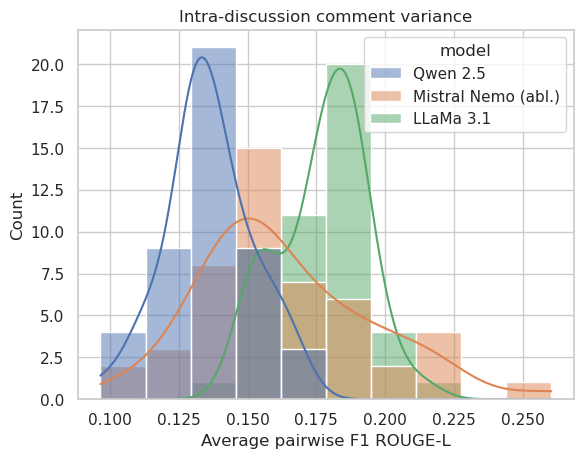
\includegraphics[width=\columnwidth]{discussion_variance.png}
	\caption{Histogram of the average pairwise F1 ROUGE-L \cite{lin-2004-rouge} scores for each discussion split by the \ac{LLM} that produced it. The score is computed by computing the F1 ROUGE-L scores for each comment in the discussion with the rest, then averaging them. Less is better (a larger ROUGE-L score indicates less variance in the discussion).}
	\label{fig::discussion_variance}
\end{figure}

%\noindent\textbf{\ac{LLM} moderators overuse positive reinforcement. However, unlike human users, the \ac{LLM} user-agents don't react adversely.}

%Intervening in comments that are relatively high-quality, by means of positive reinforcement, is a technique frequently used by human moderators \citep{falk-etal-2021-predicting}. However, intervening too much, risks alienating the users \citep{schaffner_community_guidelines, make_reddit_great, proactive_moderation}. This behavior is not observed in the synthetic discussions; the users will happily let the moderator intervene again and again, even in situations where his presence is not necessary.

%\noindent\textbf{\ac{LLM} user-agents use a relatively narrow range of behaviors when compared to humans. Giving hints for realistic behavior in the instruction prompt solves this problem, but raises questions about the authenticity of the experiments}

%Humans in online space showcase a wide breadth of behaviors, each of which interacts uniquely with the behavior of other humans. In contrast, \ac{LLM} user-agents behave in a stereotypically polite, inoffensive and analytical fashion.

%In these experiments, we added a clause in the instruction prompts to indicate that repeated provocations should not be left unanswered. We observed that now \ac{LLM} user-agents can be successfully goaded by trolls, leading to larger variance within the discussions. However, each of these clauses adds our own biases to the simulation, meaning that the \ac{LLM} user-agent behavior quickly becomes what we expect to see, rather than what we would see in the real world.


%\noindent\textbf{The inclusion of sociodemographic prompts usually leads to more varied and realistic discussions}

%As pointed out above, \ac{LLM} user-agents frequently draw from their sociodemographic background to enhance the discussion with personal anecdotes and experiences. Sometimes these are shallow comparisons, but oftentimes they are useful both for differentiating participants and for expanding the discussion in new directions. The only notable issue is that \ac{LLM} participants may mention their SDB excessively, compared to human online users. 
